\documentclass{article}
\usepackage{tkz-graph}
\usepackage{paralist}
\pagestyle{empty}
\usetikzlibrary{patterns}

\begin{document}

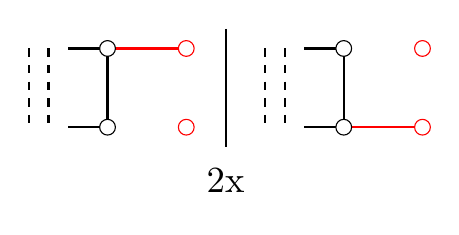
\begin{tikzpicture}

\draw[thick,dashed] ( 0, 0) -- ( 0,-1);
\draw[thick,dashed] (0.25, 0) -- (0.25,-1);

\draw[thick,-] ( 0.5, 0) -- ( 1, 0);
\draw[thick,-] ( 1, 0) -- ( 1,-1);
\draw[thick,-] ( 0.5,-1) -- ( 1,-1);

\filldraw[draw=red, thick] ( 1, 0) -- (2, 0);
%\filldraw[draw=red, thick] ( 1,-1) -- (2,-1);

\filldraw[fill=white, draw=black] ( 1, 0) circle (0.1cm);
\filldraw[fill=white, draw=black] ( 1,-1) circle (0.1cm);

\filldraw[fill=white, draw=red] ( 2, 0) circle (0.1cm);
\filldraw[fill=white, draw=red] ( 2,-1) circle (0.1cm);

	\draw[thick] (2.5, 0.25) -- (2.5,-1.25);

\draw[thick,dashed] (3, 0) -- ( 3,-1);
\draw[thick,dashed] (3.25, 0) -- (3.25,-1);

\draw[thick,-] ( 3.5, 0) -- ( 4, 0);
\draw[thick,-] ( 4, 0) -- ( 4,-1);
\draw[thick,-] ( 3.5,-1) -- ( 4,-1);

%\filldraw[draw=red, thick] ( 4, 0) -- (5, 0);
\filldraw[draw=red, thick] ( 4, -1) -- (5,-1);

\filldraw[fill=white, draw=black] ( 4, 0) circle (0.1cm);
\filldraw[fill=white, draw=black] ( 4,-1) circle (0.1cm);

\filldraw[fill=white, draw=red] ( 5, 0) circle (0.1cm);
\filldraw[fill=white, draw=red] ( 5,-1) circle (0.1cm);

\draw (2.5,-2) -- (2.5,-2) node[anchor=south, scale=1.33] {2x};

\end{tikzpicture}

\end{document}